\addcontentsline{toc}{part}{Examens précédents}

\addcontentsline{toc}{chapter}{Examen de juin 2019}

\chapter{Juin 2019}

\paragraph{Question 1} \textit{Théorie.} \\

\begin{enumerate}
\item Énoncer le postulat de la mesure. \\

\ans{ 
On rappelle qu'à toute grandeur classique $A$ correspond un opérateur hermitien $\hat A$ qui agit sur l'espace de Hilbert des états du système physique.  Cet opérateur peut s'écrire 
$\hat A = \sum_a a \hat \Pi_a$ où $a$ sont les valeurs propres de 
$\hat A$ et $\Pi_a$ les projecteurs sur les espaces propres correspondants.

Les valeurs propres (qui sont forcement réelles) de cet opérateur sont les résultats de la
mesure. Le résultat d'une telle mesure est aléatoire, et la probabilité d'obtenir une valeur propre $a$ est donnée par $P(a) = \langle \psi | \hat \Pi_a \vert \psi \rangle$ où $\ket{\psi}$ est l'état du système. 

Immédiatement après la mesure, l'état $\ket{\psi}$ est projeté sur l'état $\Pi_a \vert \psi \rangle/ \sqrt{\langle \psi | \hat \Pi_a \vert \psi \rangle} $.
Par conséquent, après la mesure, toute autre mesure  de $\hat A$ redonnera le résultat $a$ avec certitude. L'acte de la mesure quantique est donc un processus irréversible.
}

\item Soit un système à spin $1/2$. Une base de l'espace de Hilbert associé est $\lbrace\ket{\uparrow},\ket{\downarrow}\rbrace$, qui sont les états propres de $\sigma_z$ de valeurs propres $+1$ et $-1$ respectivement. 

Soit le vecteur unitaire $\vec n = (\cos \theta,\sin\theta\sin\phi,\sin\theta\cos\phi)$. Soit $\ket{\uparrow_{\vec n}}$ l'état du spin polarisé dans la direction $\vec n$. Donner l'état $\ket{\uparrow_{\vec n}}$ dans la base $\lbrace\ket{\uparrow},\ket{\downarrow}\rbrace$. \\

\ans{ 
Si on suppose que la question posée donne les composantes
dans le répère (x,y,z) comme suit
$n_x=\sin\theta\cos\phi$, $n_y=\sin\theta\sin\phi$, $n_z=\cos \theta$, alors la réponse est:

$\ket{\uparrow_{\vec n}} = \cos \theta/2 \ket{\uparrow} + \exp (i \phi) \sin \theta/2 \ket{\downarrow}$.
}

\end{enumerate}


\newpage

\paragraph{Question 2} \textit{Oscillateur harmonique quantique.} \\

Considérons un oscillateur harmonique de pulsation propre $\omega$. En unités sans dimensions ($\hbar=1$), les opérateurs position $\hat X$ et impulsion $\hat P$ obéissent à la relation de commutation canonique $[\hat X, \hat P]=i $. \\

Les opérateurs de création et destruction sont définis par 
$\hat a= \frac{1}{\sqrt{2}}(\hat X+i\hat P)$, $a^\dagger= \frac{1}{\sqrt{2}}(\hat X-i\hat P)$ et satisfont donc $[\hat a,\hat a^\dagger]=1$. \\

L'opérateur nombre $\hat N$ est donné par $\hat N= \hat a^\dagger \hat a$ et ses vecteurs propres sont notés $\hat N \ket{n} =n \ket{n}$ où $n \in \mathbb{N}$. On peut montrer que $\hat a \ket{n} =\sqrt{n} \ket{n-1}$ et que $\hat a^\dagger \ket{n} =\sqrt{n+1} \ket{n+1}$. L'hamiltonien de l'oscillateur harmonique est $\hat H = \frac{1}{2}\omega ( \hat P^2 + \hat X^2 )\ $. \\

Soit l'état quantique 
\begin{equation}
\vert \psi \rangle = 
 \frac{1}{\sqrt{3}}\ket{1} -  \frac{\sqrt{2}}{\sqrt{3}}\ket{2}   \ .
 \label{Eq:psi}
\end{equation}

\begin{enumerate}
\item 
Que vaut $\braket{\psi|\hat P|\psi}$ ? \\

\ans{
On commence par déterminer l'élément de matrice $\braket{m|\hat P|n}$ en représentation de Fock. En calculant la différence entre les définitions de $\hat a$ et $\hat a^\dagger$, il vient $\hat P = -\frac{i}{\sqrt{2}}(\hat a - \hat a^\dagger)$ et l'action des opérateurs d'échelle $\hat a$ et $\hat a^\dagger$ a été rappelée dans l'énoncé. On a donc
\begin{equation}
\hat P \ket{n} = -\frac{i}{\sqrt{2}}(\hat a \ket{n}-\hat a^\dagger \ket{n}) = -i\sqrt{\frac{n}{2}}\ket{n-1} + i\sqrt{\frac{n+1}{2}} \ket{n+1}, \, \forall\, n\in\mathbb{N}.
\end{equation}
Les vecteurs $\ket{n}$ sont vecteurs propres de l'opérateur hermitien $\hat N$, ils forment donc une base orthonormée de l'espace des états, $\braket{m|n} = \delta_{m,n}$, et satisfont donc une relation de fermeture
\begin{equation}
\sum_{m=0}^\infty \ket{m}\bra{m} = \hat I. \label{eq:FockClosure}
\end{equation}
On obtient donc
\begin{equation}
\begin{split}
\braket{m|\hat P|n} &= -i\sqrt{\frac{n}{2}}\braket{m|n-1} + i\sqrt{\frac{n+1}{2}} \braket{m|n+1} \\
&= -i\sqrt{\frac{n}{2}}\delta_{m,n-1} + i\sqrt{\frac{n+1}{2}} \delta_{m,n+1}, \, \forall\, m,n\in\mathbb{N}.
\end{split}
\end{equation}
La représentation matricielle de l'opérateur $\hat P$ dans la base $\lbrace\ket{n}\rbrace_{n\in\mathbb{N}}$ est ainsi
\begin{equation}
P = \frac{i}{\sqrt{2}} \left[
\begin{array}{ccccc}
0 & -\sqrt{1} & 0 & 0 & \cdots \\
\sqrt{1} & 0 & -\sqrt{2} & 0 & \cdots \\
0 & \sqrt{2} & 0 & -\sqrt{3} & \cdots \\
0 & 0 & \sqrt{3} & 0 & \cdots \\
\vdots & \vdots & \vdots & \vdots & \ddots
\end{array}
\right].
\end{equation}
On écrit maintenant l'état $\ket{\psi} = \frac{1}{\sqrt{3}} \sum_{k=0}^2 \alpha_k \ket{k}$ où $[\alpha_k] = [0,1,-\sqrt{2}]^T$. Alors
\begin{equation}
\begin{split}
\braket{\psi|\hat P|\psi} &= \frac{1}{3} \sum_{m,n=0}^2 \bar\alpha_m \alpha_n \braket{m|\hat P|n} \\
&= -\frac{i}{3\sqrt{2}} \sum_{m,n=0}^2 \alpha_m \alpha_n (\sqrt{n}\delta_{m,n-1} - \sqrt{n+1}\delta_{m,n+1}) \\
&= -\frac{i}{3} (\alpha_1\alpha_2 - \alpha_1\alpha_2) = \boxed{ 0 }
\end{split}
\end{equation}
Le calcul direct dans la représentation matricielle est également possible, en considérant la restriction de $\hat X$ au sous-espace engendré par $\lbrace\ket{0},\ket{1},\ket{2}\rbrace$.
\begin{equation}
\braket{\psi|\hat P|\psi} = \frac{i}{3\sqrt{2}} \Big[
\begin{array}{ccc}
0 & -1 & -\sqrt{2}
\end{array}
\Big]
\left[
\begin{array}{ccc}
0 & -\sqrt{1} & 0  \\
\sqrt{1} & 0 & -\sqrt{2} \\
0 & \sqrt{2} & 0 
\end{array}
\right]
\left[
\begin{array}{c}
0 \\
-1 \\
-\sqrt{2}
\end{array}
\right] = 0.
\end{equation}
}

\item 
Supposons qu'à l'instant $t=0$, l'oscillateur harmonique est dans l'état $\ket{\psi}$ donné par l'équation \eqref{Eq:psi}. Quel est son état $\ket{\psi(t)}$ à l'instant $t>0$ ? \\

\ans{
Pour un système conservatif, la solution générale de l'équation de Schrödinger $i\frac{d}{dt}\ket{\psi(t)} = \hat H\ket{\psi(t)}$ est donnée par $\ket{\psi(t)} = \hat U(t,t_0) \ket{\psi(t_0)}$ où $\hat U(t,t_0)$ est l'opérateur (unitaire) d'évolution défini par $\hat U(t,t_0) \equiv e^{-i\hat H (t-t_0)}$. Ce dernier est diagonal dans la base des états propres d'énergie et s'écrit
\begin{equation}
\hat U(t,t_0) = \sum_{n=0}^\infty e^{-i E_n (t-t_0)} \ket{n}\bra{n}. \label{eq:EvolutionOp}
\end{equation}
En termes des opérateurs d'échelle, l'hamiltonien (dans l'ordre normal) s'écrit 
\begin{equation}
\hat H = \frac{1}{2}\omega (\hat a^\dagger \hat a + \hat a\hat a^\dagger) = \frac{1}{2}\omega (2 \hat a^\dagger \hat a + [\hat a,\hat a^\dagger]) = \omega \Big(\hat N + \frac{1}{2}\Big) \Rightarrow E_n = \omega\Big(n+\frac{1}{2}\Big).
\end{equation}
Si l'on fixe l'origine du temps à $t_0 = 0$ et que l'on fait agir l'opérateur \eqref{eq:EvolutionOp} sur l'état \eqref{Eq:psi}, il vient immédiatement, grâce au caractère orthonormal de la base
\begin{equation}
\boxed{
\ket{\psi(t)} = \frac{1}{\sqrt{3}} \Big[ e^{-\frac{3}{2} i \omega t } \ket{1}  - \sqrt{2} e^{-\frac{5}{2} i \omega t } \ket{2} \Big].
}
\end{equation}
%On voit que les probabilités de mesurer les valeurs d'énergie $E_n$ dans l'état $\ket{\psi(t)}$ sont identiques à celles concernant l'état $\ket{\psi}$ initial. Ceci est dû au caractère unitaire de l'évolution des états (Postulat 5). 
}

\item 
Calculer les éléments de matrice $\braket{m|\hat X^2|n}$ pour tout $m,n\in \mathbb{N}$. \\

\ans{
On peut obtenir l'expression de $\hat X$ en fonction des opérateurs d'échelle en sommant leurs définitions respectives : $\hat X = \frac{1}{\sqrt{2}}(\hat a+\hat a^\dagger)$. On peut alors calculer explicitement $\hat X^2 = \frac{1}{2}(\hat a+\hat a^\dagger)^2$ que l'on exprime sous forme normale
\begin{equation}
\begin{split}
\hat X^2 &= \frac{1}{2} \Big( \hat a^2+ (\hat a^\dagger)^2 + \hat a^\dagger \hat a + \hat a \hat a^\dagger \Big) \\
&= \frac{1}{2} \Big( \hat a^2+ (\hat a^\dagger)^2 + 2 \hat a^\dagger \hat a + [\hat a, \hat a^\dagger] \Big) \\
&= \frac{1}{2} \Big( \hat a^2+ (\hat a^\dagger)^2 + 2 \hat a^\dagger \hat a + 1\Big).
\end{split}
\end{equation}
	L'opérateur $\hat a$ détruit une excitation de l'oscillateur, tant et si bien que l'élément de matrice $\braket{m|\hat a^2|n}$ ne sera non-nul qu'à condition que $n = m+2$ car $\hat a^2 \ket{n} \propto \ket{n-2}$ et $\braket{m|n-2} = \delta_{m,n-2}$. De manière symétrique, l'élément de matrice $\braket{m|(\hat a^\dagger)^2|n}$ sera non-nul à condition que $n = m-2$. Quant à $\braket{m|(2\hat a^\dagger \hat a + 1)|n}$, l'opérateur inséré détruit puis crée une excitation. Par conséquent, seul l'élément diagonal $m=n$ sera non-nul. Comme les différents termes présentent des éléments de matrice non-triviaux pour des configurations différentes du couple $(m,n)$, il est très facile de recenser les seuls éléments de matrice $\braket{m|\hat X^2|n}$ qui sont non-nuls. Il s'agit de
\begin{equation}
\boxed{ 
\begin{split}
\braket{n-2|\hat X^2|n} &= \frac{1}{2} \braket{n-2|\hat a^2|n} = \frac{1}{2}\sqrt{n(n-1)}, \\
\braket{n+2|\hat X^2|n} &= \frac{1}{2} \braket{n+2|(\hat a^\dagger)^2|n} = \frac{1}{2} \sqrt{(n+1)(n+2)}, \\
\braket{n|\hat X^2|n} &= \frac{1}{2} \braket{n|(2\hat a^\dagger \hat a + 1)|n} = \braket{n|\hat N|n} + \frac{1}{2} = \frac{1}{2} (2n+1), \, \forall n \in\mathbb{N}.
\end{split}
}
\end{equation}
}

\newpage
\item Utiliser le résultat de l'exercice précédent pour évaluer $\braket{n|\hat X^4|n}$ pour tout $n\in \mathbb{N}$. \\

\ans{
Connaissant les éléments de matrice de $\hat X^2$ dans la base de Fock, les éléments diagonaux de $\hat X^4$ se déduisent aisément grâce à la relation de fermeture \eqref{eq:FockClosure} :
\begin{equation}
\begin{split}
\braket{n|\hat X^4|n} = \braket{n|\hat X^2\,{\color{red}\hat I}\,\hat X^2|n} &= {\color{red}\sum_{m=0}^\infty} \bra{n}\hat X^2{\color{red}\ket{m}\bra{m}}\hat X^2\ket{n} \\
&= \sum_{m=0}^\infty \Big|\braket{m|\hat X^2|n}\Big|^2 \\
&= \Big|\braket{n-2|\hat X^2|n}\Big|^2 +  \Big|\braket{n+2|\hat X^2|n}\Big|^2 + \Big|\braket{n|\hat X^2|n}\Big|^2 \\
&= \frac{1}{4} \Big[ n(n-1) + (n+1)(n+2) + (2n+1)^2 \Big] \\
&= \boxed{ \frac{3}{4} (2n^2 + 2n +1).}
\end{split}
\end{equation}
%Ce qui termine l'exercice !
}

\end{enumerate}

\newpage

\paragraph{Question 3} \textit{Résonance quantique de l'ion carbonate.} \\

\begin{figure}[h!]
\begin{center}
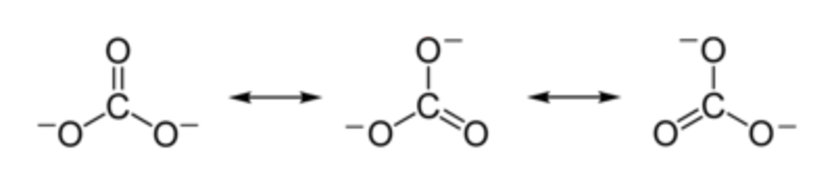
\includegraphics[width=0.8\columnwidth]{Pictures/Carbonate1.pdf} 
\end{center}
\caption{L'ion carbonate. L'atome de carbone a une liaison double vers un atome d'oxygène, et deux liaisons simples vers 2 ions oxygène. Ceci résulte en 3 configurations possibles que nous noterons $\vert 1 \rangle$, $\vert 2 \rangle$, et $\vert 3 \rangle$, entre lesquelles la molécule peut faire des transitions.
}
\label{fig:Carbonate1}
\end{figure}

\begin{figure}[h!]
\begin{center}
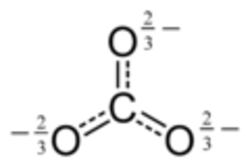
\includegraphics[width=0.2\columnwidth]{Pictures/Carbonate2.pdf} 
\quad \quad
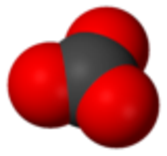
\includegraphics[width=0.13\columnwidth]{Pictures/Carbonate3.pdf} 
\end{center}
\caption{A gauche : une représentation de l'ion carbonate qui respecte la symétrie de la molécule. Les charges négatives sont délocalisées. A droite : une représentation à 3 dimension en termes du volume occupé par chaque atome.
}
\label{fig:Carbonate2}
\end{figure}



L'ion carbonate (voir figure \ref{fig:Carbonate1}) a la formule chimique CO$_3^{2-}$. C'est une molécule plane, avec l'atome de carbone au centre. Naïvement, l'atome de carbone devrait avoir une liaison double (plus courte) vers un atome d'oxygène, et deux liaisons simples (plus longues) vers 2 ions oxygène. Mais ceci brise la symétrie de la molécule, qui a 3 liaisons de même longueur, et 3 atomes d'oxygène équivalents. La symétrie observée expérimentalement (voir figure \ref{fig:Carbonate2}) peut s'expliquer par le phénomène de résonance quantique. \\

Les 3 configurations possibles de l'ion carbonate sont illustrées à la Figure \ref{fig:Carbonate1}. Notons ces configurations $\vert 1 \rangle$, $\vert 2 \rangle$, et $\vert 3 \rangle$. La molécule peut effectuer des transitions entre ces configurations. Nous pouvons donc modéliser l'Hamiltonien du système par
\begin{equation}
H= E_0 \Big (\vert 1\rangle \langle 1\vert + 
\vert 2\rangle \langle 2\vert  +\vert 3\rangle \langle 3\vert  \Big)
-
A \Big( \vert 2\rangle \langle 1\vert + 
\vert 3\rangle \langle 2\vert  +\vert 1\rangle \langle 3\vert + \mathrm{h.c.} \Big)
\label{Eq:CO3}
\end{equation}
où $E_0$ est l'énergie des différentes configurations si on ne tient pas compte des transitions, les termes proportionels à $A$ tiennent compte des transitions possibles entre configurations, et ``h.c.'' veut dire ``hermitien conjugué''.
\begin{enumerate}

\newpage
\item Quelles sont les énergies des 3 états propres de l'Hamiltonien $H$ défini par l'équation \eqref{Eq:CO3} (en termes des paramètres $E_0$ et $A$) ? \\

\ans{
Dans la base $\lbrace\ket{1},\ket{2},\ket{3}\rbrace$ des états de configuration électronique de l'ion carbonate, l'opérateur hermitien $\hat H$ se représente par la matrice
\begin{equation}
H = \left[
\begin{array}{ccc}
E_0 & -A & -A \\
-A & E_0 & -A \\
-A & -A & E_0
\end{array}
\right].
\end{equation}
L'hermiticité de $\hat H$ implique que les paramètres $E_0$ et $A$ sont des nombres réels. Les valeurs propres $\lambda$ de $H$ vérifient l'équation caractéristique $\det (H - \lambda I) = 0$ qui se simplifie en
\begin{equation}
\begin{split}
&\lambda^3 - 3 E_0 \lambda^2 + (3 E_0^2-3A^2)\lambda + (2A^3+3A^2E_0 - E_0^3) = 0 \\
&\Leftrightarrow (E_0 +A -\lambda)^2 (E_0 -2 A - \lambda) = 0.
\end{split}
\end{equation}
Nous obtenons deux valeurs propres 
\begin{equation}
\boxed{ \lambda_+ = E_0+A \text{ et } \lambda_- = E_0 - 2 A }
\end{equation}
de multiplicités algébriques respectives $\mu_A^+ = 2$ et $\mu_A^- = 1$.\\

\textbf{Note pratique sur l'organisation du calcul :} pour trouver les racines du polynôme caractéristique à la main, un raccourci de notation évident est de poser $\xi \equiv \lambda - E_0$. On obtient alors une équation cubique en $\xi$ qui est $\xi^3 - 3 A^2 \xi + 2 A^3=0$. On remarque immédiatement que les solutions seront de la forme $\xi = \sigma A$ (car alors, les 3 termes de l'équation sont tous cubiques en $A$). Il faut donc trouver $\sigma$ comme solution de $\sigma^3 - 3 \sigma + 2 = 0$. On peut essayer des entiers, et on constate que $\sigma = 1$ et $\sigma = -2$ conviennent. Il suffit ensuite d'écrire l'équation caractéristique sous la forme $(\sigma - 1)(\sigma + 2)(\sigma - \sigma_0) = 0$, et déterminer $\sigma_0$ pour reproduire le polynôme caractéristique. On obtient $\sigma_0 = 1$ en annulant le terme quadratique qui n'existait pas dans ce polynôme. On obtient donc $(\sigma-1)^2 (\sigma + 2) = 0$. \hfill $\square$
}

\item Quels sont les états propres de $\hat  H$ ? \\

\ans{
Comme $H$ est symétrique réelle, elle est nécessairement diagonalisable par transformation orthogonale et donc la multiplicité géométrique $\mu_G$ de toute valeur propre est égale à sa multiplicité algébrique. Ainsi, $\mu_G^+ = \mu_A^+ = 2$ on s'attend donc à trouver 2 vecteurs linéairement indépendants associés à $\lambda_+$. 
\begin{equation}
H - \lambda_+ I = -A \left[
\begin{array}{ccc}
1 & 1 & 1 \\
1 & 1 & 1 \\
1 & 1 & 1 
\end{array}
\right] \Rightarrow 
\ket{\lambda_+} = \alpha \ket{1} + \beta \ket{2} - (\alpha+\beta)\ket{3}.
\end{equation}
On peut se donner, à partir de là, deux vecteurs propres orthogonaux qui formeront la base du sous-espace propre de $\lambda_+$. Nous les noterons $\ket{\lambda_+^{(1)}}$ et $\ket{\lambda_+^{(2)}}$. Considérons, par exemple, la classe de vecteurs avec $\beta = 0$. Ils sont colinéaires au vecteur normé
\begin{equation}
\ket{\lambda_+^{(1)}} \equiv \frac{1}{\sqrt{2}} (\ket{1} - \ket{3}).
\end{equation}
On construit maintenant
\begin{equation}
\ket{\lambda_+^{(2)}} \equiv \alpha' \ket{1} + \beta' \ket{2} - (\alpha'+\beta')\ket{3}.
\end{equation}
et on ajuste $\alpha'$ et $\beta'$ tels que $\braket{\lambda_+^{(1)}|\lambda_+^{(2)}} = 0$ et $\braket{\lambda_+^{(2)}|\lambda_+^{(2)}} = 1$. La première condition donne $2\alpha'+\beta'=0$ ce qui détermine $\beta'$. $\alpha'$ est fixé par la seconde condition qui impose que $2(\alpha'^2 +\alpha'\beta'+\beta'^2) = 6\alpha'^2 = 1$, soit $\alpha' = \frac{1}{\sqrt{6}}$. Le vecteur
\begin{equation}
\ket{\lambda_+^{(2)}} = \frac{1}{\sqrt{6}} ( \ket{1} -2 \ket{2} + \ket{3}).
\end{equation}
convient ainsi pour compléter la base orthonormée du sous-espace $M_+ \equiv \ker \, (\hat H - \lambda_+ \hat I)$. Le dernier vecteur propre est associé à $\lambda_-$ :
\begin{equation}
H - \lambda_- I = -A \left[
\begin{array}{ccc}
-2 & 1 & 1 \\
1 & -2 & 1 \\
1 & 1 & -2 
\end{array}
\right] \Rightarrow 
\ket{\lambda_-} = \frac{1}{\sqrt{3}} (\ket{1} +  \ket{2} +\ket{3}).
\end{equation}
Une base de vecteurs propres est donc
\begin{equation}
\boxed{
\begin{split}
\ket{\lambda_-} &= \frac{1}{\sqrt{3}} (\ket{1} + \ket{2} + \ket{3}), \\
\ket{\lambda_+^{(1)}} &= \frac{1}{\sqrt{2}} (\ket{1} - \ket{3}), \\
\ket{\lambda_+^{(2)}} &= \frac{1}{\sqrt{6}} (\ket{1} - 2 \ket{2} + \ket{3}). \\
\end{split}
}
\end{equation}
Cette base n'est bien évidemment pas unique, et seulement définie à transformations orthogonales près à l'intérieur du sous-espace $M_+$ !
}

\end{enumerate}

\newpage


\paragraph{Question 4} \textit{Particule confinée sur un cercle.} \\

\begin{center}
\begin{tikzpicture}[scale=0.75]
\draw (2,2) circle (3cm);
\draw[dashed] (2,2) -- (5,2);
\node at (3.5,1.7) {$R$};
\end{tikzpicture}
\end{center}

Considérons une particule de masse $m$ confinée sur un cercle de rayon $R$ et de circonférence $L=2 \pi R$. (Plus précisément, il y a un potentiel qui confine la particule dans les directions transverses. Ce potentiel est tellement fort qu'aux échelles d'énergie que nous envisageons, le seul degré de liberté est le mouvement le long du cercle). \\

Soit $x\in[-\frac{L}{2},\frac{L}{2}[$ la coordonnée le long du cercle. Le potentiel est nul tout le long du cercle $V(x)=0$. L'équation de Schrödinger stationnaire pour la particule est donc
\begin{equation}
-\frac{\hbar^2}{2m} \frac{d^2}{d x^2} \psi(x) = E \psi(x)\ .\label{eq:FreeSchrodinger}
\end{equation}
L'origine $x=0$ est choisie arbitrairement, puisque ce système possède une symétrie de rotation.
\begin{enumerate}
\item Quelles sont les conditions de raccord en $x=\pm \frac{L}{2}$ qu'il faut imposer à $\psi(x)$ pour respecter la symétrie du problème ? \\

\ans{
Un cercle de circonférence $L>0$ correspond à la droite réelle repliée sur elle-même où les points $x$ et $x+L$ ont été identifiés. La fonction d'onde définie sur ce cercle doit donc respecter cette périodicité, soit $\psi(-\frac{L}{2}) = \psi(\frac{L}{2})$
et $\frac{d}{d x}\psi(-\frac{L}{2}) = \frac{d}{d x} \psi(\frac{L}{2})$
.
} 

\item Trouver les niveaux d'énergie de la particule confinée sur un cercle, ainsi que la dégénérescence des niveaux, et donner les fonctions d'onde propres de l'hamiltonien. \\

\ans{
On résout l'équation \eqref{eq:FreeSchrodinger} pour la fonction $\psi(x)$. L'espace des solutions est un espace vectoriel de dimension 2 de fonctions réelles à valeurs complexes dont une base est donnée par
\begin{equation}
\psi_+ (x) = \alpha_+ e^{ikx}, \quad \psi_- (x) = \alpha_- e^{-ikx}, \quad k \equiv \sqrt{\frac{2mE}{\hbar^2}} \in \mathbb{R}^+ \label{eq:GenSol}
\end{equation}


Pour trouver les valeurs de $k$ compatibles avec les conditions aux bords, nous pouvons procéder de plusieurs manières.

\begin{itemize}[label=$\rhd$]
\item \textbf{Méthode 1 : argument de parité}. \\
L'Hamiltonien (en tenant compte des conditions aux bords) commute avec l'opérateur parité. Nous pouvons donc choisir les états propres pairs et impairs. Ceux ci sont:
\begin{equation}
\psi_{\text{pair}} (x) = A_p \cos {kx}, \quad \psi_{\text{impair}} (x) = A_i \sin{kx}, \quad k \equiv \sqrt{\frac{2mE}{\hbar^2}} \in \mathbb{R}^+. \label{eq:GenSolPair}
\end{equation}
Les solutions doivent être périodiques de période $L$, ce qui fixe
$k L = 2 \pi n$, $n \in \mathbb{N}$. \\

\item \textbf{Méthode 2 : résolution directe des conditions de raccord}. \\
Nous considérons la solution d'énergie $E$ qui est combinaison linéaire des 2 solutions fondamentales données en \eqref{eq:GenSol} :
\begin{equation}
\psi(x) = \alpha_+ e^{ikx} + \alpha_- e^{-ikx}\ .
\end{equation}
Les conditions aux bords donnent:
\begin{eqnarray}
\psi\Big(-\frac{L}{2}\Big)=\psi\Big(\frac{L}{2}\Big) &\Leftrightarrow & 
 \alpha_+ e^{-\frac{ikL}{2}} + \alpha_- e^{+\frac{ikL}{2}} =  \alpha_+ e^{ +\frac{ikL}{2}} + \alpha_- e^{-\frac{ikL}{2}}\nonumber\\
 \psi'\Big(-\frac{L}{2}\Big)= \psi' \Big(\frac{L}{2}\Big) &\Leftrightarrow & 
 ik\left( \alpha_+ e^{-\frac{ikL}{2}} - \alpha_- e^{+\frac{ikL}{2}} \right)= ik\left(  \alpha_+ e^{+\frac{ikL}{2}} - \alpha_- e^{-\frac{ikL}{2}}\right)\nonumber
\end{eqnarray}
Prenant des combinaisons linéaires des ces équations, nous obtenons
\begin{equation}
\left.
\begin{array}{ccc}
 \alpha_+ e^{-\frac{ikL}{2}}  &=&  \alpha_+ e^{+\frac{ikL}{2}} 
 \\
  \alpha_- e^{+\frac{ikL}{2}} &=&  \alpha_- e^{-\frac{ikL}{2}} 
\end{array}
\right\rbrace \Rightarrow e^{ikL} = 1,
\end{equation}
ce qui impose également que
$ k L = 2\pi n$, $n \in \mathbb{N}$.
\end{itemize}

Imposer une condition de raccord conduit donc à la quantification des niveaux d'énergie. On donne à présent les états propres du système :
\begin{equation}
E_n = \frac{\hbar^2 k_n^2}{2m} = \frac{2\pi^2 \hbar^2 n^2}{m L^2}, \quad \psi_\pm^{(n)} (x) = \frac{1}{\sqrt{L}} e^{\pm \frac{2\pi i}{L}n \, x}.
\end{equation}
L'état fondamental $n=0$ n'est pas dégénéré, tandis que les états excités $n>0$ sont doublement dégénérés. Ceci est dû au fait que la particule libre sur le cercle peut s'y mouvoir dans le sens trigonométrique, ou dans le sens horlogique.
}


\end{enumerate}